
%% $Id$

\chapter{Presenting theories}

\section{Generating theory browsing information} \label{sec:info}
\index{theory browsing information|bold}

Isabelle is able to generate theory browsing information, such as HTML
documents that show a theory's definition, the theorems proved in its
ML file and the relationship with its ancestors and descendants. HTML
is the hypertext markup language used on the World Wide Web to
represent text containing links to other documents.  These documents
may be viewed using Web browsers like Netscape or Lynx.

Besides the three HTML files that are made for every theory
(definition and theorems, ancestors, descendants), Isabelle stores
links to all theories in an index file. These indexes are themself
linked with other indexes to represent the hierarchic structure of
Isabelle's logics.

In addition to the HTML files, Isabelle also generates \emph{graph}
files that represent the theory hierarchy of a logic.  These graphs
can be comfortably displayed by a graph browser Java applet embedded
in the generated HTML pages. There is also a stand-alone version of
the graph browser which allows browsing theory graphs without having
to start a Web browser first. This version also includes features such
as generating {\sc PostScript} files, which are not available in the
applet version. The graph browser will be described later in this
chapter.

\medskip To generate theory browsing information for logics that are
part of the Isabelle distribution, simply append ``\texttt{-i true}''
to the \settdx{ISABELLE_USEDIR_OPTIONS} setting before making a logic.
For example, to generate browsing information for {\FOL}, first add
something like this to your Isabelle settings file:
\begin{ttbox}
ISABELLE_USEDIR_OPTIONS="-i true"
\end{ttbox}
Then \texttt{cd} into the \texttt{src/FOL} directory of the Isabelle
distribution and do \texttt{isatool make} (or even \texttt{isatool
  make all}).

\medskip The directory in which to store theory browsing information
is determined by the \settdx{ISABELLE_BROWSER_INFO} setting.

\medskip As some of Isabelle's logics are based on others (e.g. {\tt
  ZF} on {\tt FOL}) and because the HTML files list a theory's
ancestors, you should not make HTML files for a logic if the HTML
files for the base logic do not exist. Otherwise some of the hypertext
links might point to non-existing documents.

The entry point to all logics is the {\tt index.html} file located in
the directory denoted by \texttt{ISABELLE_BROWSER_INFO}.

A complete HTML version of all distributed Isabelle object-logics and
examples may be accessed on the WWW at:
\begin{ttbox}
http://www4.informatik.tu-muenchen.de/~isabelle/library/
\end{ttbox}
Of course, this is not necessarily consistent with your local version!

To present your own theories on the WWW, simply copy the whole
\texttt{ISABELLE_BROWSER_INFO} directory to your WWW server.


\section{Extending or adding a logic}

If you add a new subdirectory to Isabelle's logics (or add a
completely new logic), provide a {\tt ROOT.ML} file which reads in the
theory files. The {\tt ROOT.ML} file will then be processed via the
function

\begin{ttbox}\index{*use_dir}
use_dir : string -> unit
\end{ttbox}

which takes a path as its parameter, changes the working directory,
executes {\tt ROOT.ML}, and makes sure that theory browsing
information is generated properly. The {\tt index.html} file written
in this directory will be automatically linked to the first index
found in the (recursively searched) super directories.

The \texttt{usedir} utility (see also \S\ref{sec:tool-usedir}) will
automatically take care of this.

\medskip The generated HTML files contain all theorems that were
proved in the theory's \ML{} file with {\tt qed}, {\tt qed_goal} and
{\tt qed_goalw}, or stored with {\tt bind_thm} and {\tt store_thm}.
Additionally, there is a hypertext link to the whole \ML{} file.

You can add section headings to the list of theorems by using

\begin{ttbox}\index{*use_dir}
section: string -> unit
\end{ttbox}

in a theory's ML file, which converts a plain string to a HTML heading
and inserts it before the next theorem proved or stored with one of
the above functions.


%\section*{*Using someone else's database}
%
%To make them independent from their storage place, the HTML files only
%contain relative paths which are derived from absolute ones like the
%current working directory, {\tt gif_path} or {\tt base_path}. The
%latter two are reference variables which are initialized at the time
%when the {\tt Pure} database is made. Because you need write access
%for the current directory to make HTML files and therefore (probably)
%generate them in your home directory, the absolute {\tt base_path} is
%not correct if you use someone else's database or a database derived
%from it.
%
%In that case you first should set {\tt base_path} to the value of {\em
%your} Isabelle main directory, i.e. the directory that contains the
%subdirectories where standard logics like {\tt FOL} and {\tt HOL} or
%your own logics are stored. If you do not do this, the generated HTML
%files will still be usable but may contain incomplete titles and lack
%some hypertext links.
%
%It's also a good idea to set {\tt gif_path} which points to the
%directory containing two GIF images used in the HTML documents.
%Normally this is the \texttt{src/Tools} subdirectory of Isabelle's
%main directory. While its value in general is still valid, your HTML
%files would depend on files not owned by you. This prevents you from
%changing the location of the HTML files (as they contain relative
%paths) and also causes trouble if the database's maker (re)moves the
%GIFs.
%
%Here's what you should do before invoking {\tt init_html} using
%someone else's \ML{} database:
%
%\begin{ttbox}
%base_path := "/home/someone/Isabelle-dist/src";
%gif_path := "/home/someone/Isabelle-dist/src/Tools";
%init_html();
%\dots
%\end{ttbox}


\section{Browsing theory graphs} \label{sec:browse}
\index{theory graph browser|bold} 

The graph browser is a tool for visualizing dependency graphs of
Isabelle theories. Certain nodes of the graph (i.e.~theories) can be
grouped together in ``directories'', whose contents may be hidden,
thus enabling the user to filter out irrelevant information.  The
browser is written in Java, it can be used both as a stand-alone
application and as an applet.


\subsection{Invoking the graph browser}

The stand-alone version of the graph browser is wrapped up as an
Isabelle tool called \tooldx{browser}:
\begin{ttbox}
Usage: browser [GRAPHFILE]
\end{ttbox}
When no filename is specified, the browser automatically changes to
the directory \texttt{ISABELLE_BROWSER_INFO/graph/data}.

\medskip The applet version of the browser can be invoked by opening
the {\tt index.html} file in the directory
\texttt{ISABELLE_BROWSER_INFO} from your Web browser and selecting
``version for Java capable browsers''.  There is also a link to the
corresponding theory graph in every logic's {\tt index.html} file.


\subsection{Using the graph browser}

The browser's main window, which is shown in figure
\ref{browserwindow}, consists of two subwindows: In the left
subwindow, the directory tree is displayed. The graph itself is
displayed in the right subwindow.
\begin{figure}[h]
  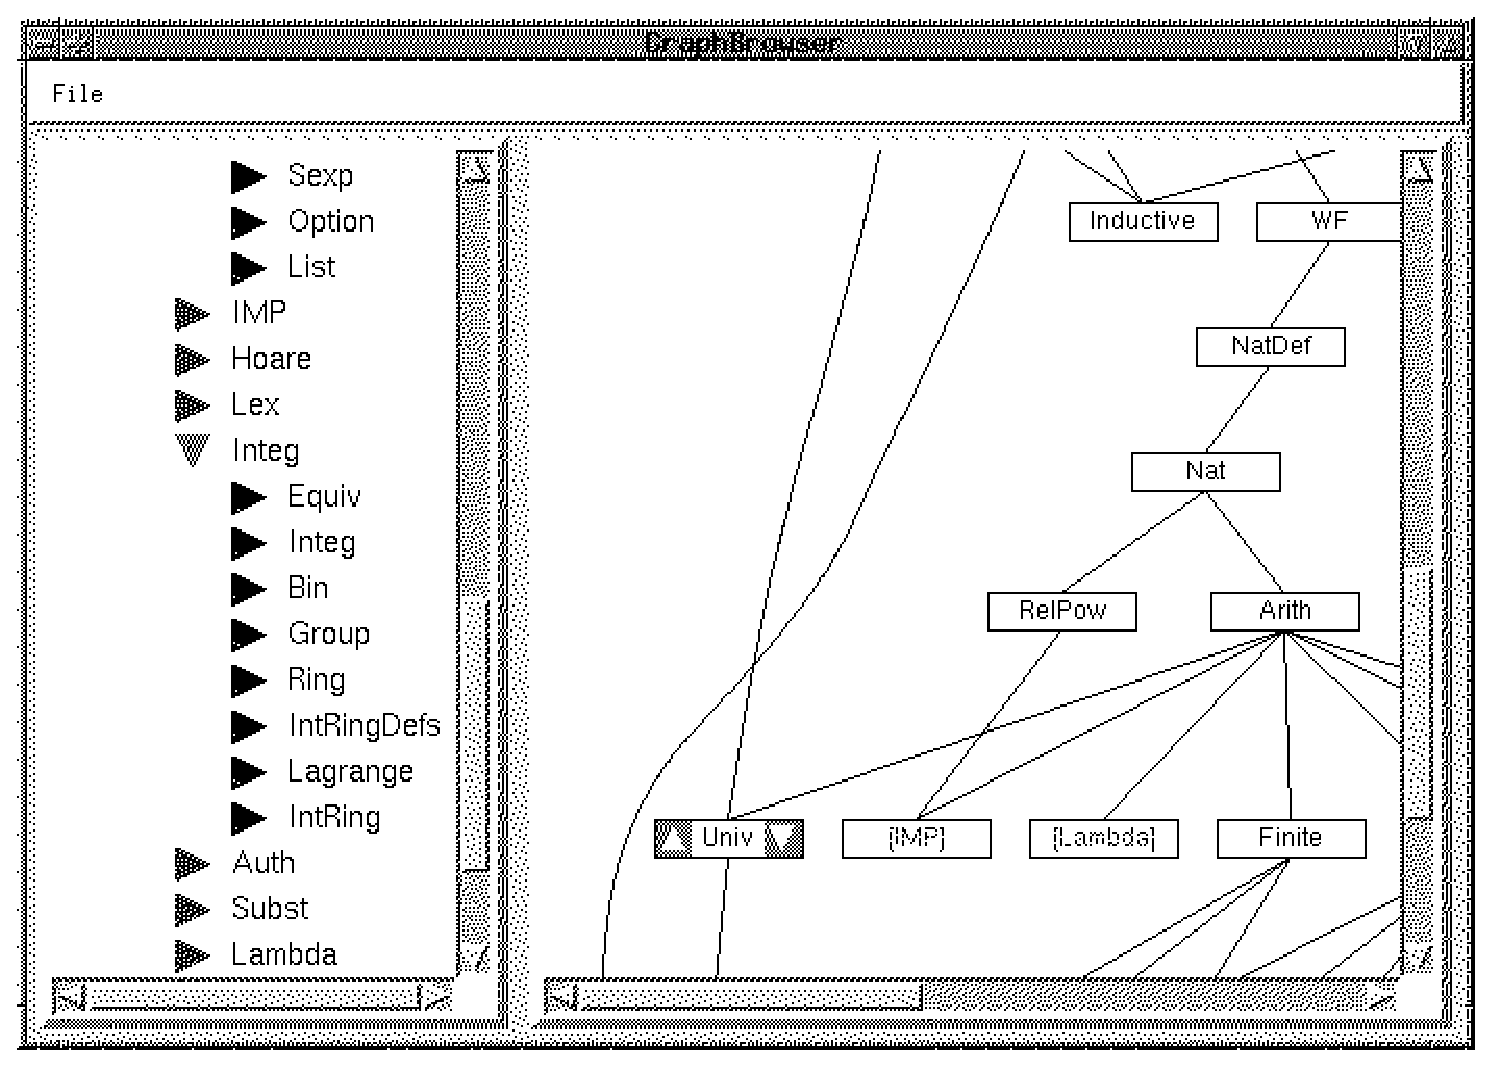
\includegraphics[width=\textwidth]{browser_screenshot.eps}
  \caption{\label{browserwindow} Browser main window}
\end{figure}


\subsubsection*{The directory tree window}

This section describes the usage of the directory browser and the
meaning of the different items in the browser window.
\begin{itemize}
  
\item A red arrow before a directory name indicates that the directory
  is currently ``folded'', i.e.~the nodes in this directory are
  collapsed to one single node. In the right subwindow, the names of
  nodes corresponding to folded directories are enclosed in square
  brackets and displayed in red colour.
  
\item A green downward arrow before a directory name indicates that
  the directory is currently ``unfolded''. It can be folded by
  clicking on the directory name.  Clicking on the name for a second
  time unfolds the directory again.  Alternatively, a directory can
  also be unfolded by clicking on the corresponding node in the right
  subwindow.
  
\item Blue arrows stand before ordinary node (i.e.~theory) names. When
  clicking on such a name, the graph display window focuses to the
  corresponding node. Double clicking invokes a text viewer window in
  which the contents of the theory file are displayed.

\end{itemize}


\subsubsection*{The graph display window}

When pointing on an ordinary node, an upward and a downward arrow is
shown.  Initially, both of these arrows are green. Clicking on the
upward or downward arrow collapses all predecessor or successor nodes,
respectively. The arrow's colour then changes to red, indicating that
the predecessor or successor nodes are currently collapsed. The node
corresponding to the collapsed nodes has the name ``{\tt [....]}''. To
uncollapse the nodes again, simply click on the red arrow or on the
node with the name ``{\tt [....]}''. Similar to the directory browser,
the contents of theory files can be displayed by double clicking on
the corresponding node.


\subsubsection*{The ``File'' menu}

Please note that due to Java security restrictions this menu is not
available in the applet version. The meaning of the menu items is as
follows:
\begin{description}
  
\item[Open$\ldots$] Open a new graph file.
  
\item[Export to PostScript] Outputs the current graph in {\sc
    PostScript} format, appropriately scaled to fit on one single
  sheet of paper.  The resulting file can printed directly.
  
\item[Export to EPS] Outputs the current graph in Encapsulated {\sc
    PostScript} format. The resulting file can be included in other
  documents.

\item[Quit] Quit the graph browser.

\end{description}


\subsection*{*Syntax of graph definition files}

A graph definition file has the following syntax:
\begin{eqnarray*}
  \mbox{\it graph} & = & \{ \: \mbox{\it vertex \tt ;} \: \} ^ + \\
  vertex & = & \mbox{\it vertexname} \: \mbox{\it vertexID} \: \mbox{\it dirname} \: [ \mbox{\tt +} ]
  \: \mbox{\it path} \: [ \mbox{\tt <} | \mbox{\tt >} ] \: \{ \: \mbox{\it vertexID} \: \} ^ *
\end{eqnarray*}

The meaning of the items in a vertex description is as follows:
\begin{description}
  
\item[vertexname] The name of the vertex.
  
\item[vertexID] The vertex identifier. Note that there may be two
  vertices with equal names, whereas identifiers must be unique.
  
\item[dirname] The name of the ``directory'' the vertex should be
  placed in.  A ``{\tt +}'' sign after {\it dirname} indicates that
  the nodes in the directory are initially visible. Directories are
  initially invisible by default.
  
\item[path] The path of the corresponding theory file. This is
  specified relatively to the path of the graph definition file.
  
\item[List of successor/predecessor nodes] A ``{\tt <}'' sign before
  the list means that successor nodes are listed, a ``{\tt >}'' sign
  means that predecessor nodes are listed. If neither ``{\tt <}'' nor
  ``{\tt >}'' is found, the browser assumes that successor nodes are
  listed.

\end{description}
